\section{Problem (4)}

	A sphere of weight $0.084 \ N$ is suspended from a cord. A steady horizontal breeze pushes the sphere so that the cord makes a constant angle of $11^{o}$ with the vertical.

	\subsection{Question (a)}
		Find the magnitude of that push:

		\textbf{R:} \newline

		\begin{figure}[H]
			\begin{center}
				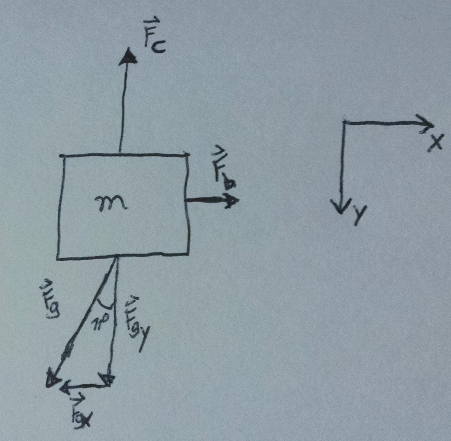
\includegraphics[scale=0.7]{hw5_problem4_fbd}
				\caption{Free-Body Diagram (Problem 4)}
				\label{fig:hw5_problem4_fbd}
			\end{center}
		\end{figure}

		Newton's $2^{nd}$ Law:
		\begin{align}
			\sum F_{x} = \ &ma_{x}& \notag \\
			F_{b} - F_{g_{x}} = \ &m(0)& \notag \\
			F_{b} = \ &F_{g_{x}}& \notag \\
			= \ &F_{g} \sin 11^{o}& \notag \\
			= \ &(0.084 \ N)(0.191)& \notag \\
			= \ &0.016 \ N&
		\end{align}

	\subsection{Question (b)}
		Find the tension in the cord:

		\textbf{R:} \newline

		Newton's $2^{nd}$ Law:
		\begin{align}
			\sum F_{y} = \ &ma_{y}& \notag \\
			F_{c} - F_{g_{y}} = \ &m(0)& \notag \\
			F_{c} = \ &F_{g_{y}}& \notag \\
			= \ &F_{g} \cos 11^{o}& \notag \\
			= \ &(0.084 \ N)(0.982)& \notag \\
			= \ &0.082 \ N&
		\end{align}
